% Create a Table of Contents in Beamer
\documentclass{beamer}[handout]
\geometry{paperwidth=150mm,paperheight=112mm}

\usetheme[subsection=false, headline=false]{INS}

%\usepackage{graphicx}
\usepackage{bbm}
\usepackage{url}
%\usepackage{tikz}
\usepackage{pgfplots}
\usetikzlibrary{arrows.meta}
\usetikzlibrary{calc}

\usepackage[linesnumbered,ruled,vlined]{algorithm2e}    % Algorithmen setzen.
\newcommand{\SkipBeforeAndAfter}{\vspace{8mm}}
%\SetAlgoSkip{SkipBeforeAndAfter}
%\SetAlgoSkip{bigskip} 
%\usepackage{algorithm}
%\usepackage{algpseudocodex}
%\algrenewcommand\algorithmicrequire{\textbf{Input:}}
%\algrenewcommand\algorithmicensure{\textbf{Output:}}
%\algnewcommand{\LeftComment}[1]{\Statex \(\triangleright\) #1}
\usepackage{amsmath,amssymb,amsthm,amsfonts,amsbsy,latexsym}    % "Notwendige" AMS-Math Pakete.
\usepackage{array}                      % Bessere Tabellen.
\renewcommand{\arraystretch}{1.15}      % Tabellen bekommen ein wenig mehr Platz.
\usepackage{bbm}                        % Dicke 1.
\usepackage[utf8]{inputenc}             % utf8 als Eingabeformat. should be loaded before biblatex
%\usepackage[backend=biber, style=alphabetic]{biblatex}  % Gute Erweiterung zu bibtex, Wird für Referenzen benutzt.
\usepackage[backend=biber, style=alphabetic]{biblatex}
%\setbeamertemplate{bibliography item}{\insertbiblabel}
\bibliography{masterthesis_your_name_bibliography.bib}   % Die verwendeten Referenzen (.bib-Datei)
\usepackage[hypcap]{caption}            % Damit Hyperrefs bei der figure-Umgebung auf die Figure zeigt statt auf die Caption.
\captionsetup{font=footnotesize} 
\usepackage{hyperref}
\usepackage{cleveref}
\usepackage{diagbox}                    % Diagonale in Tabellen.
\usepackage[T1]{fontenc}                % Bessere Schrift
\usepackage{ifthen}                     % Zum checken ob Parameter leer sind.
\usepackage{lmodern}                    % Bessere Schrift
\usepackage{listings}                   % Code Listings.
\usepackage{mathtools}                  % Subscript unter Summen behandeln. Der Befehl lautet \mathclap.
\usepackage{makeidx}                    % Stichwortverzeichnis.
\makeindex                              % Stichwortverzeichnis erstellen.
\renewcommand{\indexname}{Index}        % Name des Index definieren.
\usepackage{multirow}                   % In Tabellen mehrere Zeilen zu einer machen.
%\usepackage[parfill]{parskip}
\usepackage{rotating}                   % Um Figures zu drehen.
\usepackage{scrhack}                    % Verbessert die Zusammenarbeit von KOMA mit anderen Paketen (z.B, listing).
\usepackage{stackrel}                   % Symbole übereinander stapeln.
\usepackage[dvipsnames]{xcolor}         % Gefärbter Text und so.
\usepackage{media9}                     % für animations 
\usepackage{multimedia}

\newcommand{\bA}{\mathbb{A}}
\newcommand{\bB}{\mathbb{B}}
\newcommand{\bC}{\mathbb{C}}
\newcommand{\bD}{\mathbb{D}}
\newcommand{\bE}{\mathbb{E}}
\newcommand{\bF}{\mathbb{F}}
\newcommand{\bG}{\mathbb{G}}
\newcommand{\bH}{\mathbb{H}}
\newcommand{\bI}{\mathbb{I}}
\newcommand{\bJ}{\mathbb{J}}
\newcommand{\bK}{\mathbb{K}}
\newcommand{\bL}{\mathbb{L}}
\newcommand{\bM}{\mathbb{M}}
\newcommand{\bN}{\mathbb{N}}
\newcommand{\bO}{\mathbb{O}}
\newcommand{\bP}{\mathbb{P}}
\newcommand{\bQ}{\mathbb{Q}}
\newcommand{\bR}{\mathbb{R}}
\newcommand{\bS}{\mathbb{S}}
\newcommand{\bT}{\mathbb{T}}
\newcommand{\bU}{\mathbb{U}}
\newcommand{\bV}{\mathbb{V}}
\newcommand{\bW}{\mathbb{W}}
\newcommand{\bX}{\mathbb{X}}
\newcommand{\bY}{\mathbb{Y}}
\newcommand{\bZ}{\mathbb{Z}}

\newcommand{\bfn}{\mathbf{n}}
\newcommand{\bfx}{\mathbf{x}}
\newcommand{\bfy}{\mathbf{y}}
\newcommand{\bs}[1]{{\boldsymbol#1}}

%\newcommand{\dd}{\mathrm{d}} 
\newcommand{\dd}{\operatorname{d}\!}
\newcommand{\inv}{^{-1}}
\newcommand*{\hm}{^H}
\newcommand*{\tp}{^T}

\newcommand\cconj[1]{\mathop{\overline{#1}}}
\newcommand\closure[1]{\overline{#1}}

\DeclareMathOperator{\spn}{span}
\DeclareMathOperator{\intr}{\text{int}}
\DeclareMathOperator{\rk}{\text{rank}}
\DeclareMathOperator{\diag}{diag}
\DeclareMathOperator{\Ima}{\text{Im}}

%\DeclarePairedDelimiter{\abs}{\lvert}{\rvert}
%\DeclarePairedDelimiter{\norm}{\lVert}{\rVert}

\newcommand\comment[1]{\textcolor{magenta}{\emph{#1}}}

%\bibliographystyle{alpha}

% Title page details: 
\title[Supervisor: Prof. Dr. Jochen Garcke]{Data Visualization with t-SNE in Theory and Practice} 
%\subtitle{a proposal}
\author[Author, I.]{Solveig Tr\"ankner, Supervisor: Prof. Dr. Jochen Garcke}
%\institute[U. Bonn - INS]{University of Bonn - Institute for Numerical Simulation}
\date[Bachelor's thesis presentation]{19th December 2024}
\titlegraphic{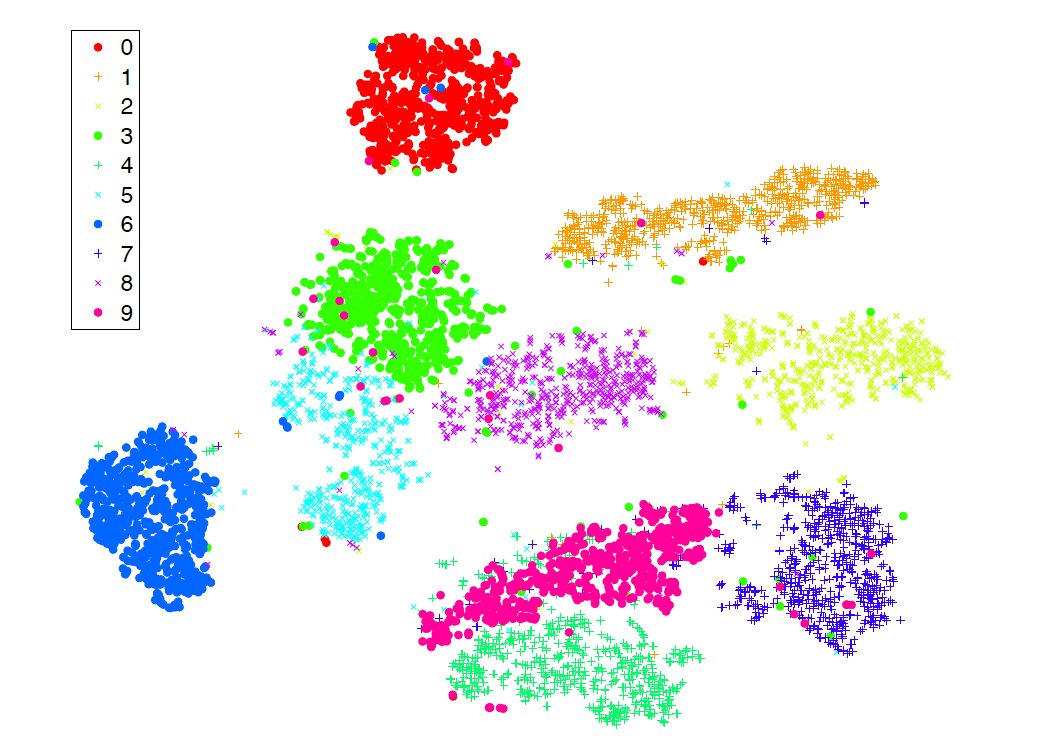
\includegraphics[width = 10cm]{tsne_title_image.png}}
\logo{\includegraphics[height = .75cm]{INS-Logo_ohne}\quad\includegraphics[height = .75cm]{uni-logo_compact.eps}}


\begin{document}
% Title page frame
\begin{frame} 
    %\vspace*{\fill}
    \titlepage
    %\begin{beamercolorbox}[sep=0.2cm,left,wd=\paperwidth]{frametitle}
        %{\usebeamerfont{title}t-Stochastic Neighbour Embeddings}

        %{\usebeamerfont{author}Solveig Tr\"ankner}

        %{\usebeamerfont{date}19th December 2024}
    %\end{beamercolorbox}
    %\vspace*{\fill}
\end{frame}
% Outline frame
\begin{frame}{Outline}
    \tableofcontents
\end{frame}

% Presentation structure
\section{Motivation}
    %\subsection{Subsections 1}

%\begin{frame}{Frametitle}{Framesubtitle}   
%\end{frame}
\begin{frame}{Dimensionality Reduction}
    \textbf{Goal}: Map high-dimensional data to a lower dimension $\mathbb{R}^d \to \mathbb{R}^s$, $s \ll d$ while perserving intrinsic structure.  \pause

    \vspace{5pt}
    \textbf{Applications}
    \begin{itemize}
        \item Compression 
        \item Feature extraction 
        \item Data visualization \pause
    \end{itemize} 
    \vspace{5pt}
    \textbf{Methods}
    \begin{itemize}
        \item Linear methods: Principal Component Analysis (PCA), Multidimensional Scaling (MDS) 
        \item Nonlinear methods: Isomap, t-Stochastic Neighbor Embedding (t-SNE)
    \end{itemize}
\end{frame}

\begin{frame}{Challenges of High Dimensions} 
    \textbf{Curse of Dimensionality}
    \begin{itemize}
        \item Volume of a hypercube (with side length $2$) grows in $\mathcal{O}(2^d)$ 
        \item Data points become sparse 
    \end{itemize}\pause
    \vspace{5pt}
    \textbf{Distance Concentration}
    \begin{itemize}
        \item In high-dimensional spaces $\frac{\lVert x_i - x_j\rVert}{\lVert x_i - x_k\rVert} \approx 1$ for most $x_i, x_j, x_k$. 
        \item Euclidean distance becomes less meaningful 
    \end{itemize}\pause
    \vspace{5pt}
    \textbf{Crowding Problem}
    \begin{itemize}
        \item High-dimensional points cannot be faithfully embedded in two or three dimensions
        \item Intrinsically distant points may cluster artificially due to limited space in the embedding 
    \end{itemize}
\end{frame}


\iffalse
\begin{frame}{Problems of sampling-based methods}
    \begin{tikzpicture} [scale=0.4,baseline=0pt]
        \draw[->] (0, 0) -- (8, 0) node[right] {$\bs{y}$};
        \draw[->] (0, 0) -- (0, 8) node[above] {$\lambda^{(\bs{y})}$};
        \draw[scale=1, domain=0:8, smooth, variable=\x, blue, dashed] plot ({\x}, {\x+3});
        \draw[scale=1, domain=0:8, smooth, variable=\y, red]  plot ({\y}, {11-\y});

        \foreach \Point in {(-2,1.5), (-1,1), (-2,3), (-1,2.5), (1,3)}{
            \node at \Point {\textbullet};
        }

        \foreach \Point in {(2,-1.5), (1,-1), (2,-3), (1,-2.5), (1,-3)}{
            \node[blue] at \Point {$\circ$};
        }
        \fill (a.base) circle[radius=.1pt];



        \draw[->] (17, 0) -- (25, 0) node[right] {$\bs{y}_1$};
        \draw[->] (17, 0) -- (14, -3) node[left] {$\bs{y}_2$};
        \draw[->] (17, 0) -- (17, 8) node[above] {$\lambda^{(\bs{y})}$};

        \draw[dashed, thick] (18,-1.5) arc (170:10:2.6cm and 0.6cm)coordinate[pos=0] (a);
        \draw[thick] (18,-1.5) arc (-170:-10:2.6cm and 0.6cm)coordinate (b);
        %\draw[densely dashed] ([yshift=4cm]$(a)!0.5!(b)$) -- node[right,font=\footnotesize] {$h$}coordinate[pos=0.95] (aa)($(a)!0.5!(b)$)
        %                        -- node[above,font=\footnotesize] {$r$}coordinate[pos=0.1] (bb) (b);
        %\draw (aa) -| (bb);
        \draw[thick] (a) -- ([yshift=3cm]$(a)!0.5!(b)$) -- (b);
        \draw[thick] (18,4.5) arc (170:10:2.6cm and 0.6cm)coordinate[pos=0] (a2);
        \draw[thick] (18,4.5) arc (-170:-10:2.6cm and 0.6cm)coordinate (b2);
        %\draw[densely dashed] ([yshift=4cm]$(a2)!0.5!(b2)$) -- node[right,font=\footnotesize] {$h$}coordinate[pos=0.95] (aa2)($(a2)!0.5!(b2)$)
        %                        -- node[above,font=\footnotesize] {$r$}coordinate[pos=0.1] (bb2) (b2);
        %\draw (aa2) -| (bb2);
        \draw[thick] (a2) -- ([yshift=3cm]$(a)!0.5!(b)$) -- (b2);
    \end{tikzpicture}
\end{frame}
\fi

\section{t-SNE}

\begin{frame}{The Main Idea Behind t-SNE}
    \begin{problem}
        Given a set of high-dimensional points $\mathcal{X} = \{x_1, x_2, ..., x_n\} \subset \mathbb{R}^d$ find a "good" lower-dimensional representation $\mathcal{Y} = \{y_1, y_2, ... , y_n\} \subset \mathbb{R}^s$ of these points, where $s=2,3$. 
    \end{problem}\pause
    \vspace{5pt}
    \textbf{An Informal Overview of t-SNE \cite[Van der Maaten, Hinton]{JMLR:v9:vandermaaten08a}}
    \begin{itemize}
        \item Create an initial set of points $\mathcal{Y}$ in $\mathbb{R}^s$ 
        \item Turn $\mathcal{X}$ and $\mathcal{Y}$ into probability distributions reflecting pairwise similarities between datapoints 
        \item Force these distributions to be as similar as possible by moving points in the lower dimension around 
    \end{itemize}
\end{frame}

\begin{frame}{Measuring Similarity of Data Points}
    \textbf{How can we measure similarity between points in a high dimension?} \pause 
    \begin{itemize}
        \item Compute a joint probability distribution over points $x_i$ and $x_j$ ($i \neq j$) via \[ 
        p_{i|j} = \frac{\exp(-||x_i-x_j||^2/2\sigma_i^2)}{\sum_{k\neq i} \exp (- ||x_i - x_k||^2/2\sigma_i^2)},\; p_{ij} = \frac{p_{i|j}+ p_{j|i}}{2n}
        \]
        where $\sigma_i$ denotes the bandwidth of the Gaussian kernel centered at $x_i$. \pause 
    \end{itemize}
    \textbf{Should we measure similarity in} $\mathbb{R}^2$ \textbf{in the same way?}  \pause 
    \begin{itemize}
        \item To avoid overcrowding, we define a similarity measure between points in the low dimensional embedding $y_i$ and $y_j$ ($i \neq j$) via \[ q_{ij} = \frac{(1+ ||y_i - y_j||^2)^{-1}}{\sum_{l} \sum_{k\neq l} (1+ ||y_k - y_l||^2)^{-1}} \]
        using a Student's t-distribution with one degree of freedom (Cauchy distribution) which is heavy-tailed compared to a Gaussian. 
    \end{itemize}
\end{frame}

\begin{frame}{Defining a Loss Function}
    \begin{definition}[Kullback-Leibler divergence]
        Let $P$ and $Q$ be discrete probability distributions defined on a sample space $\mathcal{X}$. 
        The Kullback-Leibler divergence between $P$ and $Q$ is defined as 
        \[ \text{KL}(P|| Q) = \sum_{x \in \mathcal{X}} P(x) \log \frac{P(x)}{Q(x)}.\] 
    \end{definition} \pause
    \begin{itemize}
        
        \item We want to find points $\{y_1, ..., y_n\}$ which minimize the Kullback-Leibler divergence between the distributions $P$ and $Q$ defined above. \pause
        \item The loss function is given by \[ C(\mathcal{Y}) = KL(P||Q) = \sum_{i} \sum_{j \neq i}  p_{ij} \log \frac{p_{ij}}{q_{ij}}\] \pause
        \item KL divergence is asymmetric, i.e. in general $\text{KL}(P || Q) \neq \text{KL}(Q || P)$. 
    \end{itemize}
\end{frame}

\begin{frame}{Optimization via Gradient Descent}
    \begin{itemize}
        \item We can minimize $C(\mathcal{Y})$ using Gradient Descent, where 
        \[ \frac{\partial C}{\partial y_i} = 4 \sum_{j \neq i} (p_{ij} - q_{ij}) q_{ij} Z (y_i - y_j)
        \text{ with } Z = \sum_{l} \sum_{k\neq l} (1+ \lVert y_k - y_l \rVert^2)^{-1}.\] \\ \pause 
        \item Standard optimization techniques for gradient descent can be employed, such as including a momentum term
        \[ y_i^{(t+1)} = y_i^{(t)} - h \cdot \frac{\partial C}{\partial y_i^{(t)}} + \beta (y_i^{(t)} - y_i^{(t-1)}) \text{ with } 0 \leq \beta < 1, h>0. \] \pause
        \item Rewriting the gradient yields interpretation via attractive and repulsive forces: 
        \[ -\frac{1}{4} \frac{\partial C}{\partial y_i} = \underbrace{\sum_{j\neq i} p_{ij} q_{ij} Z (y_j - y_i)}_\text{attractive force} \underbrace{-\sum_{j \neq i} q_{ij}^2 Z (y_j - y_i)}_\text{repulsive force}
        \] 
        
    \end{itemize}
\end{frame}




\section{Optimizing t-SNE}

\begin{frame}{Initialization}
    \begin{itemize}
        \item It is best to use "informative initialization" instead of random initialization for t-SNE. 
        \item PCA initialization better preserves global structure.  
    \end{itemize}
    \begin{figure}
        \centering
        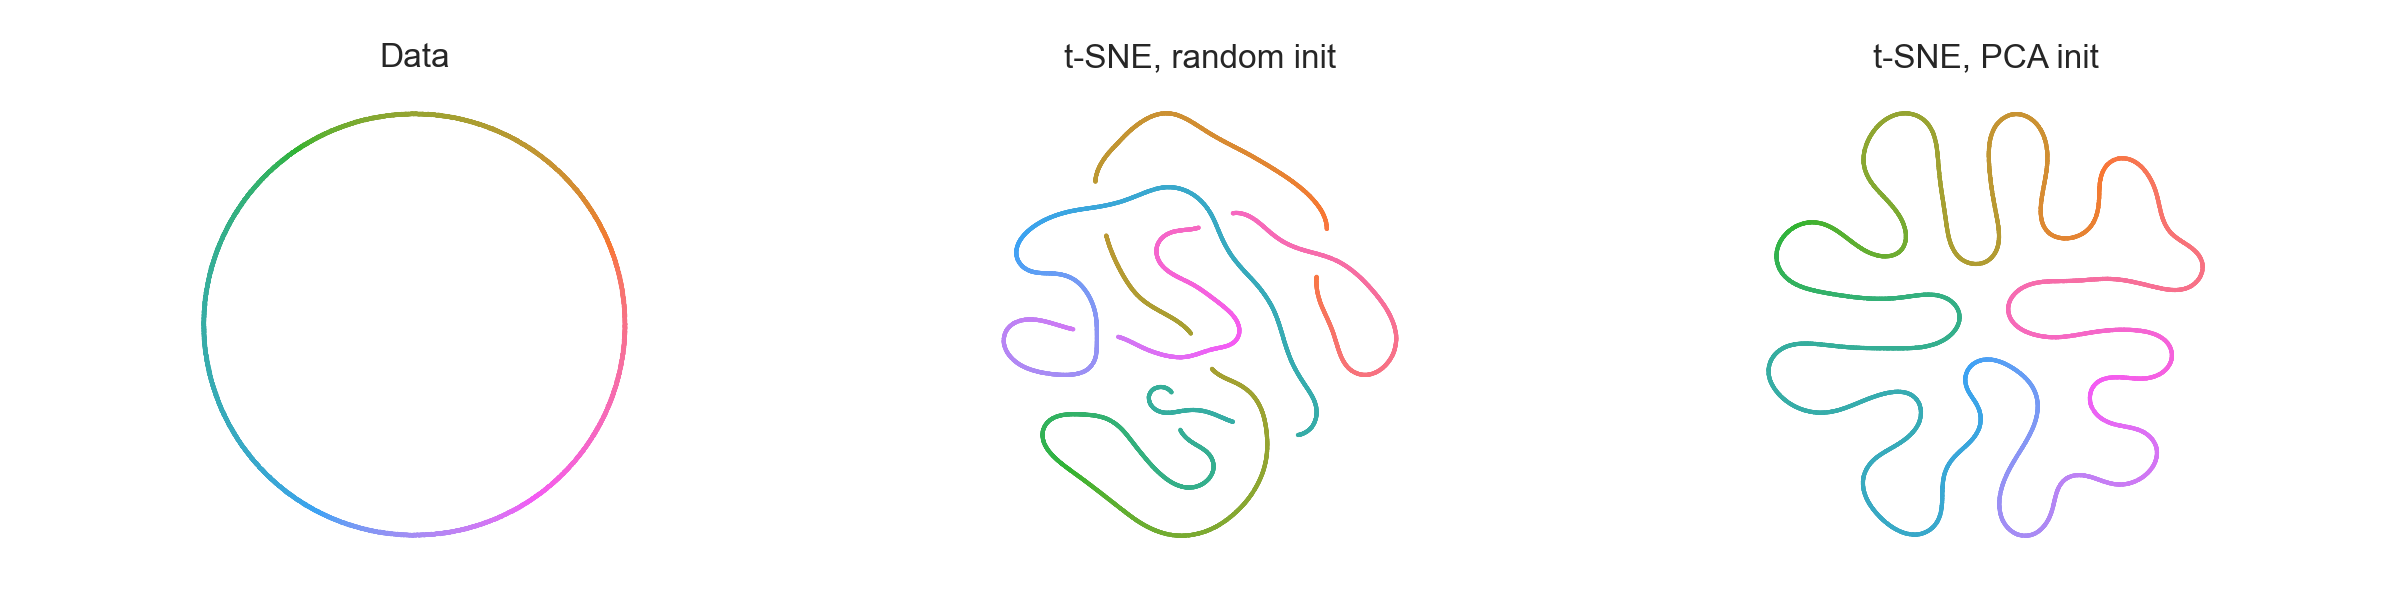
\includegraphics[width=\textwidth]{tsne-circle.png}
        \caption{The t-SNE algorithm only produces a faithful representation of the circle with informative initialization. Visualization reproduced from \cite{kl2021}}. 
    \end{figure} 
\end{frame}

\begin{frame}{Perplexity}
    \begin{itemize}
        \item Recall \[p_{i|j} = \frac{\exp(-||x_i-x_j||^2/2\sigma_i^2)}{\sum_{k\neq i} \exp (- ||x_i - x_k||^2/2\sigma_i^2)}.\] How do we choose the bandwidth $\sigma_i$ of the Gaussian kernel centered at $x_i$? \pause
        \item It depends on the data! In dense regions, we want a smaller $\sigma_i$ than in sparse ones.  \pause 
    \end{itemize}
    \begin{definition}[Shannon Entropy]
        Let $X$ be a discrete random variable taking values in $\mathcal{X}$ which is distributed according to $p: \mathcal{X} \to [0,1]$, then the Shannon Entropy is $H(X) = - \sum_{x \in \mathcal{X}} p(x) \log_2 (p(x))$.
    \end{definition}
    \begin{itemize}
        \item We define a constant \textbf{perplexity} value 
        \[ \text{Perp}(P_i) = 2^{H(P_i)} = 2^{-\sum_{j} p_{j|i} \log p_{j|i}}\] where $P_i$ is the probability distribution induced by $\sigma_i$. \pause
        \item Perplexity effectively measures the number of neighbours we wish to consider.  
    \end{itemize}
\end{frame}

\begin{frame}{Perplexity}
    \begin{figure}
        \centering
        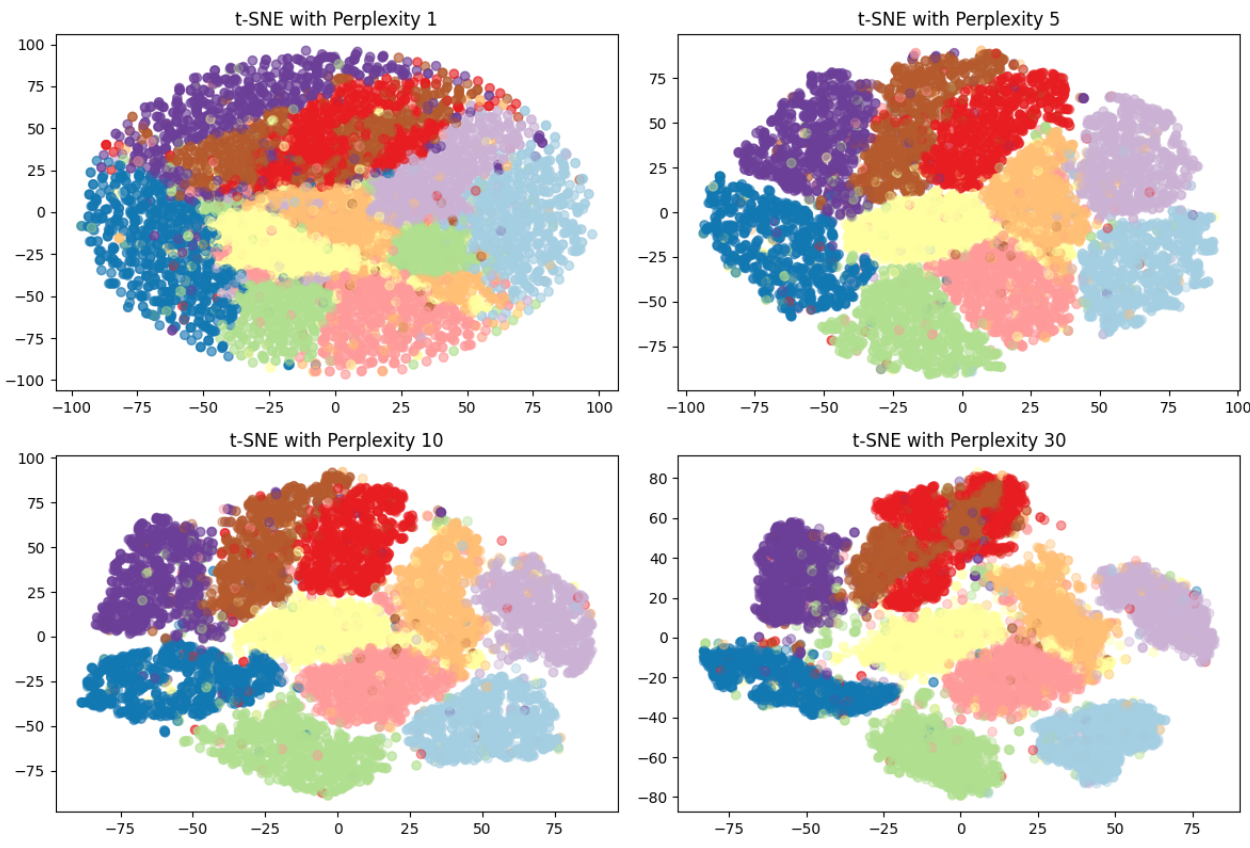
\includegraphics[width=0.8\textwidth]{varying_perplexity.png}
        \caption{Different perplexity values on the MNIST dataset.}
    \end{figure} 
\end{frame}

\begin{frame}{Perplexity}
    \begin{figure}
        \centering
        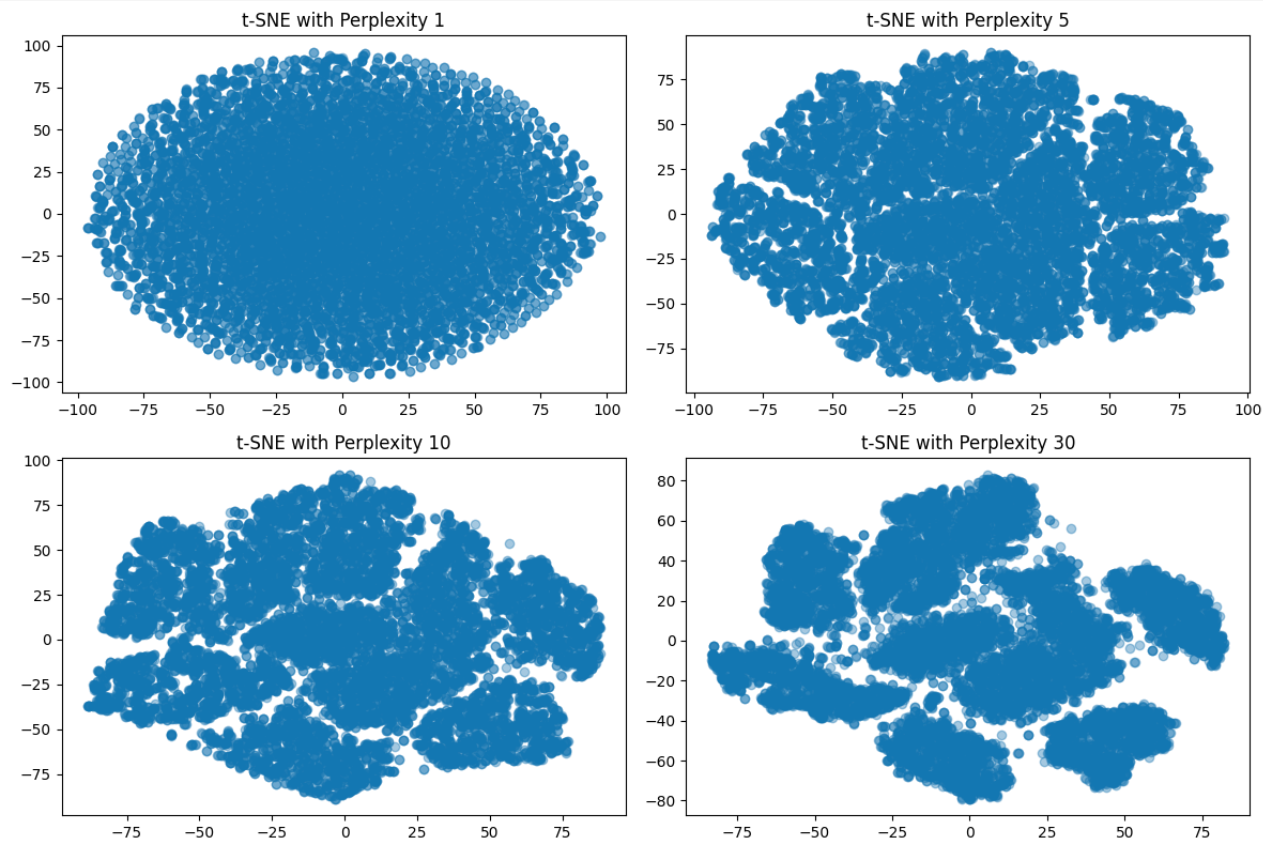
\includegraphics[width=0.83\textwidth]{perplexity_without_gt.png}
        \caption{Different perplexity values on the MNIST dataset without ground truth labels.}
    \end{figure} 
\end{frame}

\begin{frame}{Early Exaggeration}
    \begin{itemize}
        \item \textbf{Idea}: in early iterations of t-SNE we want to focus on tight cluster formation and only worry about "nice" visualization later on \pause
        \item We multiply all $p_{ij}$ by a certain factor $\alpha$ (standard value is $\alpha= 12$) for the first few iterations (standard: $250$). 
        \item Clusters can more easily move around in space later on. \pause 
        \item In the attraction-repulsion framework: 
        \[ \frac{1}{4} \frac{\partial C}{\partial y_i} = \sum_{i\neq j} \alpha p_{ij} q_{ij} Z (y_i - y_j) - \sum_{j \neq i} q_{ij}^2 Z (y_i - y_j)
        \] \pause 
        \item \textbf{Question}: How do we find good values for $\alpha$ and for how many iterations should we keep early exaggeration on? 
    \end{itemize}
\end{frame}

\begin{frame}{Automated Optimized Parameters}
    \begin{figure}
        \centering
        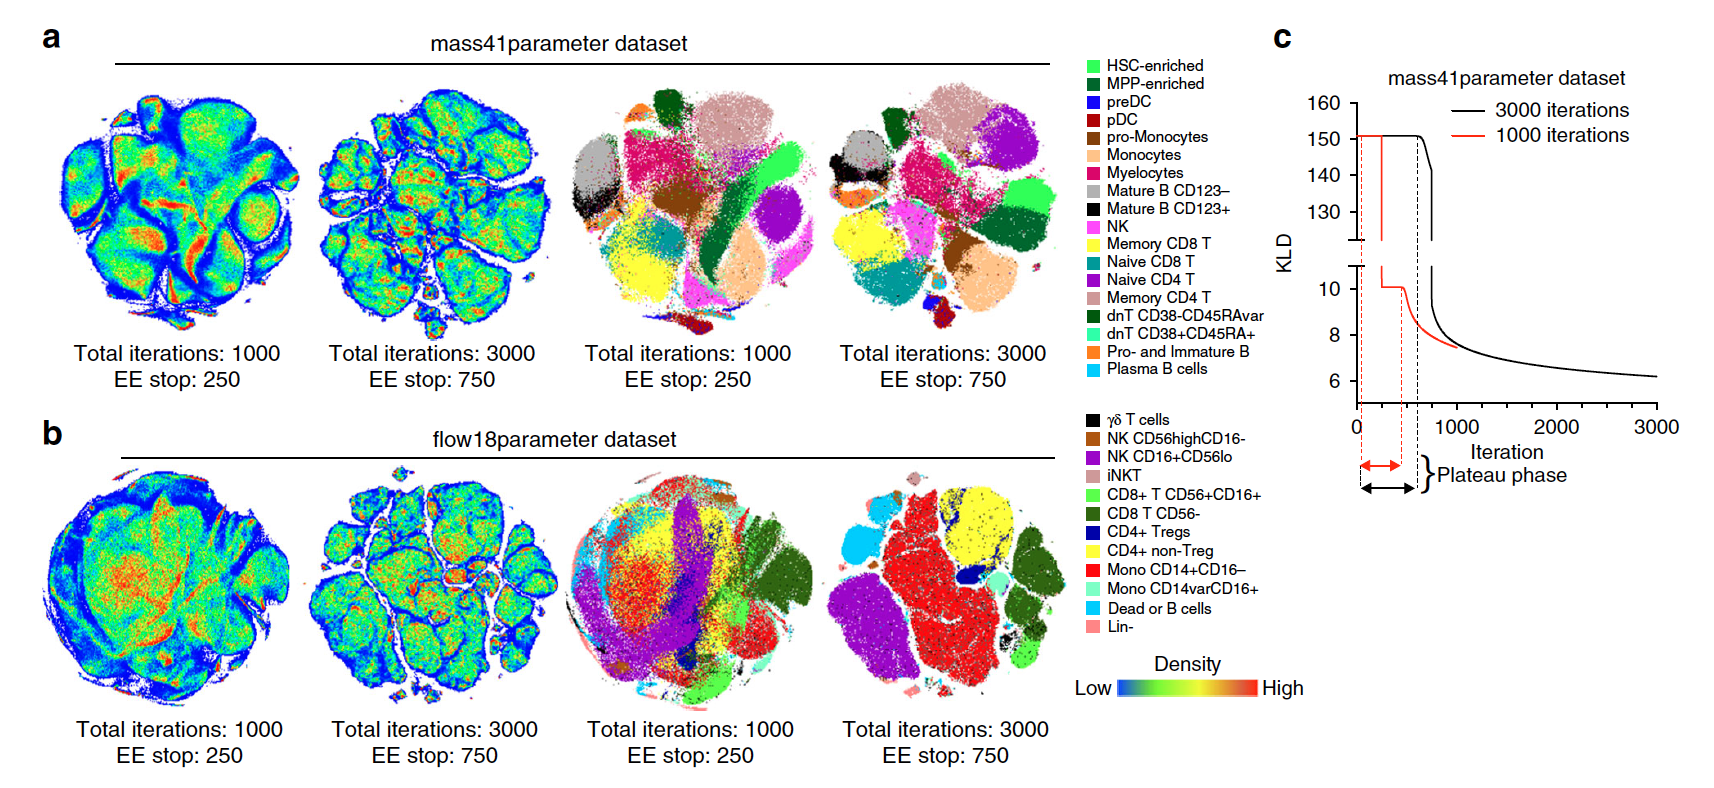
\includegraphics[width=\textwidth]{nature_EE_stop.png}
        \caption{Performance of t-SNE for cytometry data visualization, see \cite{belkina2019}.}
    \end{figure} 
\end{frame}



\section{Theoretical Results}

\begin{frame}{Theoretical Work on t-SNE}
    \begin{theorem}[Cluster Formation \cite{LindStein2022}]
        Let $\mathcal{X}$ be "clustered" and initialize $\mathcal{Y} \subset [-0.01, 0.01]^2$. Choose $\alpha$ and $h$ such that for some $1 \leq i \leq n$ \[0.01 \leq \alpha h \sum_{\substack{j \neq i \\ \text{same cluster}}} p_{ij} \leq 0.9\] Then, the diameter of the embedded cluster $\{y_i: 1 \leq j \leq n \land \pi(j) = \pi(i)\}$ decays exponentially until its diameter satisfies, for some universal $c > 0$, 
        \[ \text{diam}\{y_j: 1 \leq j \leq n \land \pi(j) = \pi(i) \} \leq c h \left( \alpha  \sum_{\substack{j \neq i \\ \text{same cluster}}} p_{ij} + \frac{1}{n}\right). \]
    \end{theorem}\pause
    \begin{itemize}
        \item Other theoretical results study connections to spectral clustering (\cite{CaiMa2022}) and limiting behaviour for $n \to \infty$ (\cite{murray2024largedatalimitsscaling}). 
    \end{itemize}
\end{frame}

\begin{frame}{Weaknesses of t-SNE}
    \begin{itemize}
        \item No convergence to global optimum guaranteed due to non-convex loss function \pause
        \item Results heavily depend on choice of parameters \pause 
        \item Visualizations can be misleading  
    \end{itemize}
    \begin{figure}
        \centering
        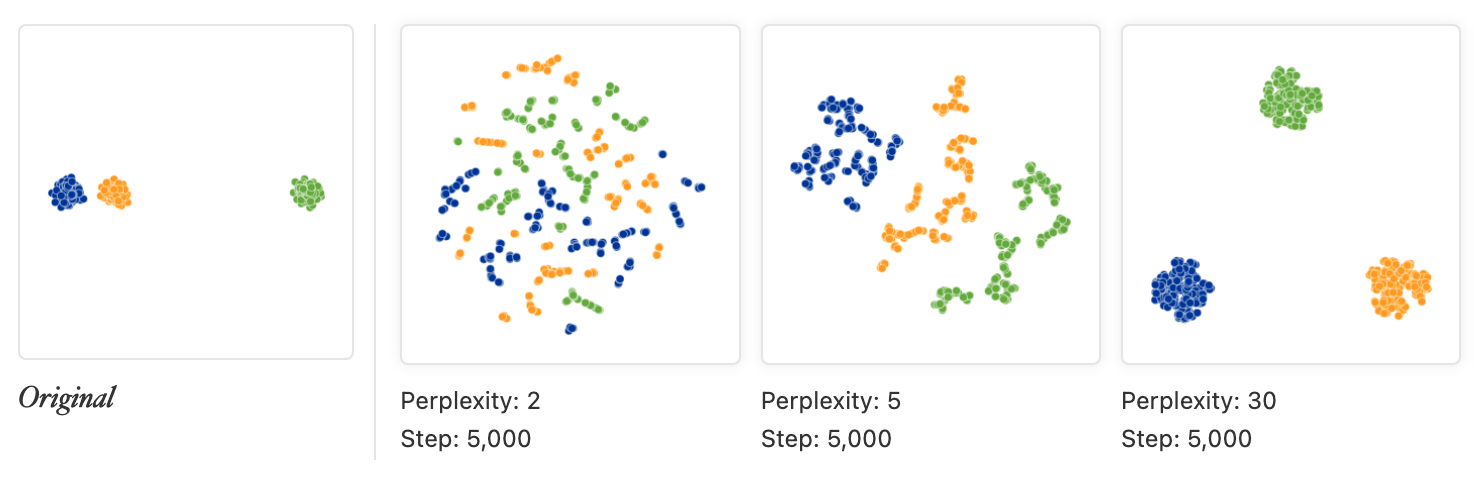
\includegraphics[width=\textwidth]{misread_tsne_1.png}
        \caption{t-SNE does not preserve distance between clusters, see \cite{wattenberg2016how}}. 
    \end{figure}
\end{frame}
 

\begin{frame}{Weaknesses of t-SNE}
    \begin{itemize}
        \item No guaranteed convergence to global optimum due to non-convex loss function 
        \item Results heavily depend on choice of parameters 
        \item Visualizations can be misleading  
    \end{itemize}
    \begin{figure}
        \centering
        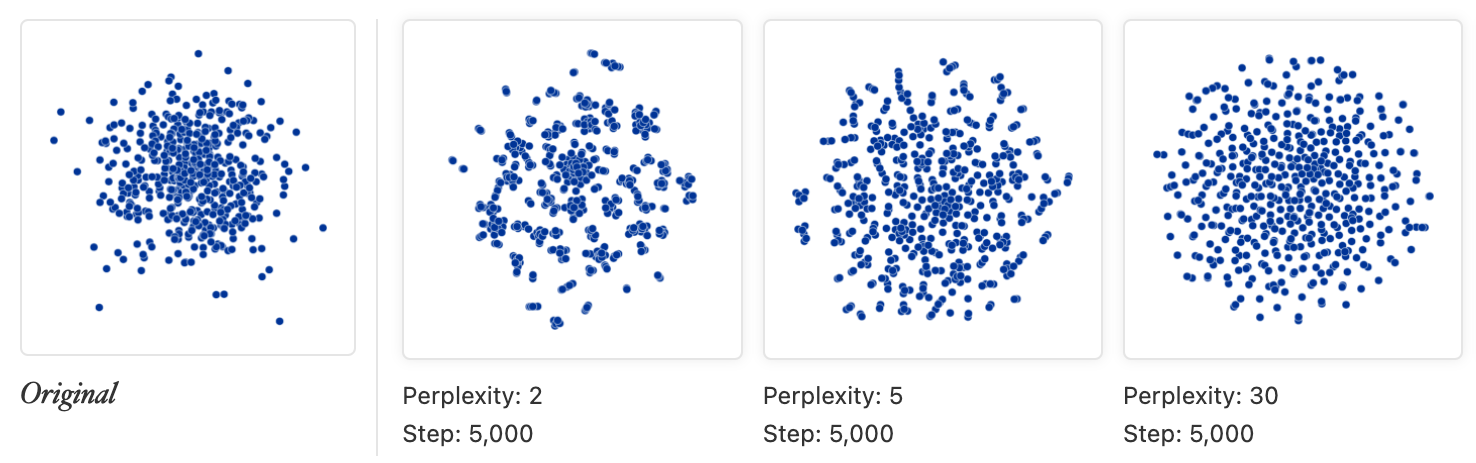
\includegraphics[width=\textwidth]{misread_tsne_2.png}
        \caption{Random Gaussian noise does not always look random, see \cite{wattenberg2016how}}. 
    \end{figure}
\end{frame}



\section{Further Questions}

\begin{frame}{Questions for Future Work}
    \begin{itemize}
        \item How realiable are theoretical results on t-SNE? Do the assumptions hold for real-world datasets? \pause
        \item Do parameters suggested in theoretical results lead to better performance in practice? \pause
        \item Which parameters are most important for obtaining good results? \pause
        \item How does initialization impact t-SNE results across different datasets? \pause
        \item How can we deal with large datasets? Does rescaled t-SNE work in practice? 
    \end{itemize}
\end{frame}

\iffalse
\begin{frame}{Blocks}
    \begin{theorem}[Sample Theorem]
        This is a theorem!
    \end{theorem} 
    \begin{lemma}[Sample Lemma]
        This is a lemma!
    \end{lemma}
    \begin{example}[Sample Example]
        This is an example!
    \end{example}
    \begin{alertblock}{Sample Alert}
        This is an alert!
    \end{alertblock}
\end{frame}

\begin{frame}{Itemize}
    \begin{itemize}
        \item Item 1
        \begin{itemize}
            \item Subitem 1
            \begin{itemize}
                \item Subsubitem 1
            \end{itemize}
        \end{itemize}
    \end{itemize}
\end{frame}
\fi

\begin{frame}[allowframebreaks]{References}
    %\nocite{*}
    \printbibliography
\end{frame}
 
\end{document}